\documentclass{book}
\usepackage{commeunjeustyle}

\begin{document}

%TODO proof  et rajouter des exemples

%%%%%%%%%%%%%%%%%%%%%%%%%%%%%%%%%%%%%%%%%%%%%%%%%%%%%%%%%%%%%%%%%%%%%%
\chapter*{Espaces vectoriels}

\section{Exemples introductifs}

\begin{Exemple}[Vecteurs du plan \(\R^2\)]
Tout d'abord, commençons par les vecteurs du plan :\\
\begin{tabular}{c|c|c|c}
 &Vecteur géométrique  &   Vecteur  numérique  &   Vecteur  algébrique       \\  \hline
Représentation&\begin{tikzpicture}[general,scale=1]
\draw [quadrillage] (-0.1,-0.1) grid (2.1,1.1);
\draw [-> ] (0,0) -- (1,0)node[right]{$\Vect{e_1}$};
\draw [->] (0,0) -- (0,1)node[right]{$\Vect{e_2}$};
\draw [->, epais,color=red] (0,0) -- (2,1)node[right]{$\Vect{u}$};
\end{tikzpicture}& $\begin{pmatrix}
2\\1
\end{pmatrix}$ & $\Vect{u}= 2 \Vect{e}_1 + 1 \Vect{e}_2 $  \\\hline
Multiplication par un scalaire &\begin{tikzpicture}[general,scale=1]
\draw [quadrillage] (-1.1,-1.1) grid (2.1,1.1);
\draw [->, ] (0,0) -- (1,0)node[right]{$\Vect{e_1}$};
\draw [->] (0,0) -- (0,1)node[right]{$\Vect{e_2}$};
\draw [->, epais,color=blue] (0,0) -- (-1,-0.5)node[above,right]{$\Vect{v}=-0,5 \Vect{u}$};
\draw [->, epais,color=red] (0,0) -- (2,1)node[right]{$\Vect{u}$};
\end{tikzpicture}   & $\begin{pmatrix}
-1\\-0,5
\end{pmatrix}=-0.5.\begin{pmatrix}
2\\1
\end{pmatrix}$  &  $\Vect{v}=-0.5.\Vect{u}$ \\\hline
Addition  &\begin{tikzpicture}[general,scale=1]
\draw [quadrillage] (-0.1,-0.1) grid (2.1,2.1);
\draw [->, ] (0,0) -- (1,0)node[right]{$\Vect{e_1}$};
\draw [->] (0,0) -- (0,1)node[right]{$\Vect{e_2}$};
\draw [->, epais,color=red] (0,0) --node[above,right]{$\Vect{u}$} (2,1);
\draw [->, epais,color=blue] (2,1) --node[right]{$\Vect{v}$} (1,2);
\draw [->, epais,color=black] (0,0) -- (1,2)node[above,left]{$\Vect{w}=\Vect{u}+\Vect{v}$};
\end{tikzpicture}  & $\begin{pmatrix}
1\\2
\end{pmatrix}=\begin{pmatrix}
2\\1
\end{pmatrix}+\begin{pmatrix}
-1\\1
\end{pmatrix}$&$ \Vect{w}= \Vect{u}+\Vect{v}$
\end{tabular}
\begin{Remarque}
Du fait de l'équivalence dans le plan et l'espace entre ces trois représentations,  géométrique,  numérique et algébrique, tout ce qui est vrai ou faux pour l'un l'est aussi pour l'autre. Savoir passer d'une représentation à l'autre est essentiel pour bien comprendre l'algèbre linéaire. 
\end{Remarque}
\end{Exemple}




\begin{Exemple}[Exemples d'ensembles de vecteurs : \(E=\{\Vect{x}\}\)]
Il existe de très nombreux ensembles  où il est possible d'effectuer une addition et une homothétie soit une combinaison linéaire, par exemples :
\begin{itemize}
\item l'ensemble des n-uplet réels : $\Vect{x}=(x_{1},x_{2},\ldots ,x_{n})$ et $E=\R^n$ et , où chaque $x_{i}$ est un réel,
%jeu vidéo: rendu d'objets dans une scène (jeux vidéos) et un vecteur d'appréciation de films 
\item l'ensemble des matrices carrés réels : $\Vect{x}=\begin{pmatrix}
a_{1,1} & a_{1,2} & \cdots & a_{1,n}\\
a_{2,1} & a_{2,2} & \cdots & a_{2,n}\\
\vdots & \vdots & \ddots & \vdots\\
a_{n,1} & a_{n,2} & \cdots & a_{n,n}\\
\end{pmatrix}$ et $E=\mathcal{M}_{n}(\R)$ , où  chaque $a_{i,j}$ est un un réel,
\item l'ensemble des solutions d'une équations différentielles linéaire d'ordre 1 homogène : $\Vect{x}=f$  et $E=\{f\in C_1 :  f'+a_{0}f=0\}$,
\item l'ensemble des polynômes réels : $\Vect{x}= a_{0}+a_{1}X^{1}+a_{2}X^{2}+\dots +a_{n}X^{n}$ et $E=\R[X]$,
\item l'ensemble des suites réels : $\Vect{x}=(u_{n})_{n\in \mathbb {N} }$ et $E=\R^{\N}$,
\item etc.
\end{itemize}
\end{Exemple}
Une stratégie efficace pour étudier ces ensembles est :
\begin{enumerate}
\item de définir une structure algébrique ayant la propriété de pouvoir effectuer des \defi{combinaisons linéaires} entre les éléments : cette structure s'appelle \defi{espace vectoriel},
\item de démontrer des énoncés sur cette structure  : ce qui est vrai ou faux dans cette structure  l'est aussi pour tous les cas particuliers. 
\end{enumerate}

%%%%%%%%%%%%%%%%%%%%%%%%%%%%%%%%%%%%%%%%%%%%%%%%%%%%%%%%%%%%%%%%%%%%%%
\section{Structure algébrique}
\begin{Definition}[Loi de composition interne : \(\Vect{x} \bigtriangleup \Vect{y}\)  ]
Soit $A$ un ensemble.\\
Une \defi{loi de composition interne}, $\bigtriangleup$, est une application qui, à deux éléments de $A$, associe un élément de $A$ :
$$ \Fonction{\bigtriangleup}{A\times A}{A}{(x,y)}{x \bigtriangleup y}.$$
\end{Definition}
\begin{Exemple}
\begin{itemize}
\item Sur $\R$, l'addition définie par $\Fonction{+}{\R\times \R}{\R}{(x,y)}{x + y}$, la soustraction $\Fonction{-}{\R\times \R}{\R}{(x,y)}{x - y}$ et la multiplication $\Fonction{-}{\R\times \R}{\R}{(x,y)}{x \times y}$ sont des lois de composition internes.
\item Soit $X$ un ensemble. Sur l'ensemble des parties de $X$, $\mathcal{P}(X)$, l'union définie par $\Fonction{\cup}{\mathcal{P}(X)\times \mathcal{P}(X)}{\mathcal{P}(X)}{(A,B)}{A \cup B}$ et l'intersection $\Fonction{\cap}{\mathcal{P}(X)\times \mathcal{P}(X)}{\mathcal{P}(X)}{(A,B)}{A \cap B}$ sont des lois de composition internes.
\end{itemize}

\end{Exemple}
\begin{Definition}[Propriétés usuelles]
On dit que $\bigtriangleup$ est
\begin{enumerate}
\item  \defi{associative} : si $\in(x,y,z)\in A^3$, $x \bigtriangleup (y \bigtriangleup z) = (x \bigtriangleup y) \bigtriangleup z$.
  On ne considèrera que des loi associatives.
\item
 \defi{commutative} : si $\forall(x,y)\in A^2$, $x \bigtriangleup y = y \bigtriangleup x$.
 \end{enumerate}
\end{Definition} 
 \begin{Exemple}
\begin{itemize}
\item Sur $\R$, l'addition et la multiplication sont commutatives et associatives. Ce n'est pas le cas de la soustraction car $1-0\neq 0-1$ et $1-(2-3)=2\neq -4= (1-2)-3.$
\item Sur  $\mathcal{P}(X)$, l'union et l'intersection sont commutatives et associatives.
\end{itemize}
\end{Exemple}
\begin{DefinitionProposition}[Inverse et élément neutre]
On dit que $\bigtriangleup$ admet \defi{un élément neutre} si $\exists e\in A$ tel que $\forall x\in A$, $x \bigtriangleup e = e \bigtriangleup x = x$.\\
Si il existe un élément $e$ vérifiant cette propriété, il est unique et on l'appelle \defi{le neutre}  de la loi $\bigtriangleup$.\\
On dit que $\bigtriangleup$ est   \defi{symétrique} (ou \defi{inverse} si loi est $\times$ , ou \defi{opposé} si la loi est $+$)
  Si $\bigtriangleup$ est une loi associative qui admet un neutre $e$, et si $x\in A$, on appelle  de $x$ pour la loi $\bigtriangleup$ tout élément $x'\in A$ tel que $x \bigtriangleup x' = x' \bigtriangleup x = e$.
  Si $\bigtriangleup$ est également associative, il existe au plus un élément $x'$ vérifiant cette propriété, et on l'appelle le \defi{symétrique}  de $x$ pour la loi $\bigtriangleup$.

\end{DefinitionProposition}

\begin{Definition}[Groupe]
Un \defi{groupe} est un couple $(G,\bigtriangleup)$ où $G$ est un ensemble et $\bigtriangleup$ une loi de composition interne sur $G$ associative, admettant un neutre et pour laquelle tout élément de $G$ admet un symétrique pour la loi $\bigtriangleup$.
Un groupe est dit \defi{abélien} ou \defi{commutatif} si la loi $\bigtriangleup$ est de plus commutative.
\end{Definition}
\begin{Exemple}[Le Groupe \((\R^n,+)\) ]
La loi d'addition sur $\R^n$ est définie par 
$$ \Fonction{+}{\R^n\times\R^n}{\R^n}{(\vec{x}=(x_1,x_2,\dots,x_n),\Vect{y}=(y_1,y_2,\dots,y_n))}{\Vect{x}+\Vect{y}=(x_1+y_1, x_2+y_2, \dots, x_n+y_n)}.$$

\begin{itemize}
\item  \defi{associative} : Soit $\Vect{x}=(x_1,x_2,\dots,x_n),\Vect{y}=(y_1,y_2,\dots,y_n),\Vect{z}=(z_1,z_2,\dots,z_n)\in\R^n .$\\
 On a :
 $$\begin{aligned}
 \Vect{x}+(\Vect{y}+\Vect{z})&=(x_1,x_2,\dots,x_n)+\left((y_1,y_2,\dots,y_n)+(z_1,z_2,\dots,z_n)\right)\\
 &=(x_1,x_2,\dots,x_n)+(y_1+z_1, y_2+z_2, \dots, y_n+z_n)\\
 &=(x_1+y_1+z_1, x_2+y_2+z_2, \dots, x_n+y_n+z_n)\\
  &=(x_1+y_1, x_2+y_2, \dots, x_n+y_n)+(z_1,z_2,\dots,z_n)\\
  &=\left((x_1,x_2,\dots,x_n)+(y_1,y_2,\dots,y_n)\right)+(z_1,z_2,\dots,z_n)\\
  &=(\Vect{x}+\Vect{y})+\Vect{z}
 \end{aligned}$$
 \item  \defi{commutative} : Soit $\Vect{x}=(x_1,x_2,\dots,x_n),\Vect{y}=(y_1,y_2,\dots,y_n)\in\R^n .$\\
 On a :
 $$\begin{aligned}
 \Vect{x}+\Vect{y}&=(x_1,x_2,\dots,x_n)+(y_1,y_2,\dots,y_n)\\
  &=(x_1+y_1, x_2+y_2, \dots, x_n+y_n)\\
  &=(y_1+x_1, y_2+x_2, \dots, y_n+x_n)\\
  &=\Vect{y}+\Vect{x}
 \end{aligned}$$
 \item  \defi{élément neutre} : Soit $\Vect{x}=(x_1,x_2,\dots,x_n)\in\R^n$\\
 Montrons que $\Vect{0}=(0,0,\dots,0)$ est l'élément neutre\\
 On a :
 $$\begin{aligned}
 \Vect{x}+\Vect{0}&=(x_1+0,x_2+0,\dots,x_n+0)\\
  &=(x_1, x_2, \dots, x_n)\\
  &=\Vect{x}
 \end{aligned}$$
  \item  \defi{symétrique} : Soit $\Vect{x}=(x_1,x_2,\dots,x_n)\in\R^n$\\
 Montrons que $-\Vect{x}=(-x_1,-x_2,\dots,-x_n)$ est l'opposé de $\Vect{x}$.\\
 On a :
 $$\begin{aligned}
 \Vect{x}+(-\Vect{x})&=(x_1,x_2,\dots,x_n)+(-x_1,-x_2,\dots,-x_n)\\
  &=(x_1-x_1, x_2-x_2, \dots, x_n-x_n)\\
  &=(0, 0, \dots, 0)\\
  &=\Vect{0}
 \end{aligned}$$
\end{itemize}
Donc $(\R^n,+)$ est un groupe commutatif.
\end{Exemple}


\begin{Definition}[Loi de composition externe : \(\lambda.\Vect{x}\)] Soit $\K$ et $A$ deux ensembles.\\ Une \defi{loi de composition externe}, $.$, est une application qui, à un élément de $\K$ et un élément de $A$, associe un élément de $A$ :
$$ \Fonction{.}{\K\times A}{A}{(\lambda,x)}{\lambda. x} $$
\end{Definition}
\begin{Exemple}[\((\R^n,.)\)]
La loi de multiplication sur $\R^n$ est définie par 
$$ \Fonction{.}{\R\times\R^n}{\R^n}{(\lambda,\Vect{x}=(x_1,x_2,\dots,x_n))}{\lambda.\Vect{x}=(\lambda.x_1, \lambda.x_2, \dots, \lambda.x_n)}.$$
Par exemple sur $\R^2$, $2.(1,-2)=(2,-4)$.
\end{Exemple}

\begin{Definition}[Corps \(\K\) : \(\R\) ou \(C\)] Dans ce cours%\samepage\footnote{%\begin{tiny}
%Un \defi{corps} (commutatif) $(K,+,\times )$ est un ensemble muni de deux lois internes possédant les propriétés suivantes :
%\begin{itemize}
%\item $(K,+)$ est un groupe abélien, dont l'élément neutre est noté $0$ ;
%\item $(K\setminus \{0\},\times )$ est également un groupe abélien, dont l'élément neutre est noté $1$ ;
%\item $\times$ est distributive par rapport à $+$.
%\end{itemize}
%\impo{Remarque} Lorsque le contexte est clair, on écrit souvent $\K$ au lieu de $(\K,+,×)$.\\
%\impo{Exemples}
%\begin{itemize}
%\item le corps des réels $\R$, des complexes $\C$, des rationnels $\Q$;
%\item si $\K$ est un corps, le corps des fractions rationnelles à coefficients dans $\K$, noté $\K(X)$;
%\item $\Q [i] = \{a+ib:(a,b)\in \Q ^2\}$;
%\item le corps des entiers modulo un nombre premier $p$, noté $\Z/p\Z$.
%\end{itemize}
%}
, un corps $\K$ désigne soit l'ensemble des nombres réels $\R$ ou soit l'ensemble des nombres complexes $\C$. 
\end{Definition}
\begin{Definition}[Espace vectoriel : \(\lambda\Vect{x}+\mu\Vect{y}\)]
Soit $\K$ un corps.\\
Un \defi{$\K$-espace vectoriel} est un triplet $(E,+,.)$ où
$+$ est une loi de composition interne sur $E$ et
$.$ est une loi de composition externe sur $E$,
vérifiant les propriétés suivantes:
\begin{enumerate}
\item $(E, +)$ est un groupe commutatif;
\item la loi $.$ est compatible avec la structure de groupe $(E, +)$, i.e.  
 \begin{enumerate}
  \item $\forall(\lambda ,\mu )\in\K^2$, $\forall \Vect{x}\in E$, $(\lambda +\mu ) . \Vect{x} = (\lambda . \Vect{x}) + (\mu . \Vect{x})$;
  \item $\forall\lambda \in\K$, $\forall(\Vect{x},\Vect{y})\in E^2$, $\lambda . (\Vect{x}+\Vect{y}) = (\lambda . \Vect{x}) + (\lambda . \Vect{y})$;
  \item $\forall\Vect{x}\in E$, $1_\K. \Vect{x} = \Vect{x}$;
  \item $\forall(\lambda ,\mu )\in\K^2$, $\forall\Vect{x}\in E$, $\lambda . (\mu . \Vect{x}) = (\lambda \mu ) . \Vect{x}$.
  \end{enumerate}
\end{enumerate}
Un élément d'un $\K$-espace vectoriel est appelé un \defi{vecteur} et est noté dans ce cours avec une flèche  $\Vect{x}$. Un élément du corps $\K$ est un \defi{scalaire} et est noté dans ce cours à l'aide d'une lettre grecque, $\lambda$.   
\end{Definition}


\begin{Exemple}

\begin{itemize}
\item les n-uplets $\K^n$ muni des lois usuelles, 
\item
  les matrices $\mathcal{M}_{n,p}(\K)$ muni des lois usuelles,
\item
 si $X$ est un ensemble et $E$ un $\K$-espace vectoriel, l'ensemble des fonctions $\mathcal{F}(X,E)$ muni des lois usuelles.
\end{itemize}
\end{Exemple}
%\begin{Proposition}[Structure de $\K $-espace vectoriel]
%$\MnpK$ possède une structure de $\K $-espace vectoriel. 
%\end{Proposition}
\section{Construire des espaces vectoriels}
\subsection{Sous-espace vectoriel : $F\subset E$ et $F$ e.v.}
\subsubsection{Définition}
\begin{DefinitionProposition}[Sous espace vectoriel]
Soit $(E,+,.)$ un $\K $-espace vectoriel et $F$ une partie de $E$.
On dit que $F$ est un \defi{sous espace vectoriel} de $E$ si
\begin{itemize}
\item
  $F$ est non vide,
\item
  $F$ est stable par $+$, i.e.   $\forall \Vect{x},\Vect{y} \in F$, $\Vect{x}+\Vect{y}\in F$,
\item
  $F$ est stable par $.$ , i.e.   $\forall \lambda \in \K $, $\forall \Vect{x} \in F$, $\lambda .\Vect{x}\in F$.
\end{itemize}
Muni des lois induites, F est alors un espace vectoriel.
\end{DefinitionProposition}
\begin{Exemple}
$F=\{(x,y)\in\R^2:x+2y=0\}$ \begin{tikzpicture}[general,scale=1]
\draw [quadrillage,loosely dashed] (-3,-2) grid (3,2);
\draw [->, ] (0,0) -- (1,0)node[right]{$\Vect{e_1}$};
\draw [->] (0,0) -- (0,1)node[right]{$\Vect{e_2}$};
\draw [-] (-3,1.5) -- (3,-1.5)node[right]{$F$};
\node[above]{$\Vect{0}$};
\end{tikzpicture} est un sous espace vectoriel de $\R^2$ 
car :
\begin{itemize}
\item \textit{non vide :}\\
$(0,0)\in \R^2$ car $0+2.0=0.$
\item \textit{stable par $+$ :}\\
Soit $\Vect{x}_1=(x_1,y_1),\Vect{x}_2=(x_2,y_2) \in F $ d'où $ x_1+2y_1=0$ et $ x_2+2y_2=0$.\\
Montrons que $\Vect{x}_1+\Vect{x}_2=(x_1+x_2,y_1+y_2)\in F$.\\
i.e. montrons que $(x_1+x_2)+2(y_1+y_2)=0$.\\
On a :
$$(x_1+x_2)+2(y_1+y_2)= x_1+2y_1 + x_2+2y_2 = 0+0 =0.$$
\item
  \textit{stable par $.$ :} \\
Soit $\lambda\in \R$ et $\Vect{x}=(x,y)\in F $ d'où $ x_1+2y_1=0$ et $ x_2+2y_2=0$.\\
Montrons que $\lambda\Vect{x}=( \lambda x,\lambda  y)\in F$.\\
i.e. montrons que $(\lambda x)+2(\lambda  y)=0$.\\
On a 
$$(\lambda x)+2(\lambda  y)= \lambda (x +2 y) = \lambda 0 =0.$$  
\end{itemize}
\end{Exemple}

\begin{Proposition}[Critère d'un sous-espace vectoriel]
Soit $E$ un $\K $-espace vectoriel et $F\subset E$.
$F$ est un sous espace vectoriel  de $E$ si et seulement si
\begin{itemize}
\item
  $\Vect{0_E}\in F$;
\item
  $\forall \lambda  \in \K $, $\forall  \Vect{x},\Vect{y} \in F$, $\lambda .\Vect{x} + \Vect{y} \in  F$.
\end{itemize}
\end{Proposition}
\subsubsection{Engendré par une famille finie :  }
$\Vectt (\Vect{x_1},\dots,\Vect{x_p})=\{\lambda_1. \Vect{x_1}+\dots + \lambda_p. \Vect{x_p} \}$
\begin{Definition}[Famille finie]
Soit $E$ un $\K $-espace vectoriel.\\
Une \defi{famille finie} de vecteurs de $E$ est un $p$-uplet $\mathcal{F} = (\Vect{x}_1,\dots,\Vect{x_p})$ formée de vecteurs de $E$, où $p\in \N$.
\end{Definition}
\begin{Definition}[Combinaison linéaire]
Avec les mêmes notations, une \defi{combinaison linéaire} de la famille $\mathcal{F}$ est un vecteur $\Vect{x} \in E$ de la forme $\Vect{x} = \lambda_1. \Vect{x_1}+\dots + \lambda_p. \Vect{x_p}$ où $\lambda_1,\dots,\lambda_p \in  \K$.\\
Les scalaires $\lambda_1,\dots,\lambda_p$ sont appelés \defi{coefficients} de la combinaison linéaire.\\
On note \defi{$\Vectt (\mathcal{F})$} l'ensemble des combinaison linéaires de la famille $(\Vect{x}_1,\dots,\Vect{x_p})$.\\
$$\Vectt (\mathcal{F})=\{ \lambda_1. \Vect{x_1}+\dots + \lambda_p. \Vect{x_p} : \lambda_1,\dots,\lambda_p \in  \K \}.$$
Par convention, $\Vectt(\emptyset)= \{\Vect{0}_E\}$.
\end{Definition}
\begin{DefinitionProposition}[Espace engendré]
Soit $E$ un $\K $-espace vectoriel et $(\Vect{x}_1,\dots,\Vect{x_p})$ une famille de vecteurs de $E$.\\
L'ensemble $\Vectt(\Vect{x}_1,\dots,\Vect{x_p})$ est un sous espace vectoriel  de $E$, appelé \defi{espace engendré} par la famille $(\Vect{x}_1,\dots,\Vect{x_p})$.
Il s'agit du plus petit (pour l'inclusion) sous espace vectoriel  de $E$ contenant $\Vect{x_1},\dots,\Vect{x_p}$.
\end{DefinitionProposition}
\begin{Exemple}[Droite vectoriel]
Lorsque que $p=1$ avec $ \Vect{x} \neq \Vect{0}$, $\Vectt(\Vect{x}) = \{\lambda .\Vect{x} : \forall \lambda  \in  \K  \}$
est la \defi{droite vectorielle} engendrée par $\Vect{x}$. On la note $\R \Vect{x}$.\\
Une droite vectorielle dans $\R ^2$ est 
\begin{center}
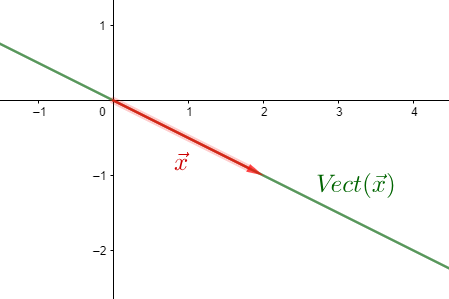
\includegraphics[width=6cm]{espace_vectoriel_droite.png}
\end{center}
\end{Exemple}
\begin{Exemple}[Plan vectoriel]
Lorsque que $p=2$ avec $ \Vect{x_1}$ non colinéaire à $\Vect{x_2}$, $\Vectt (\Vect{x_1},\Vect{x_2}) = \{\lambda .\Vect{x_1}+\mu.\Vect{x_2} : \forall \lambda ,\mu \in  \K  \}$
est le \defi{plan vectorielle} engendrée par $(\Vect{x_1},\Vect{x_2})$. On le note $\R \Vect{x_1}+\R \Vect{x_2}$.\\
Un plan vectorielle dans $\R ^3$  est 
\begin{center}
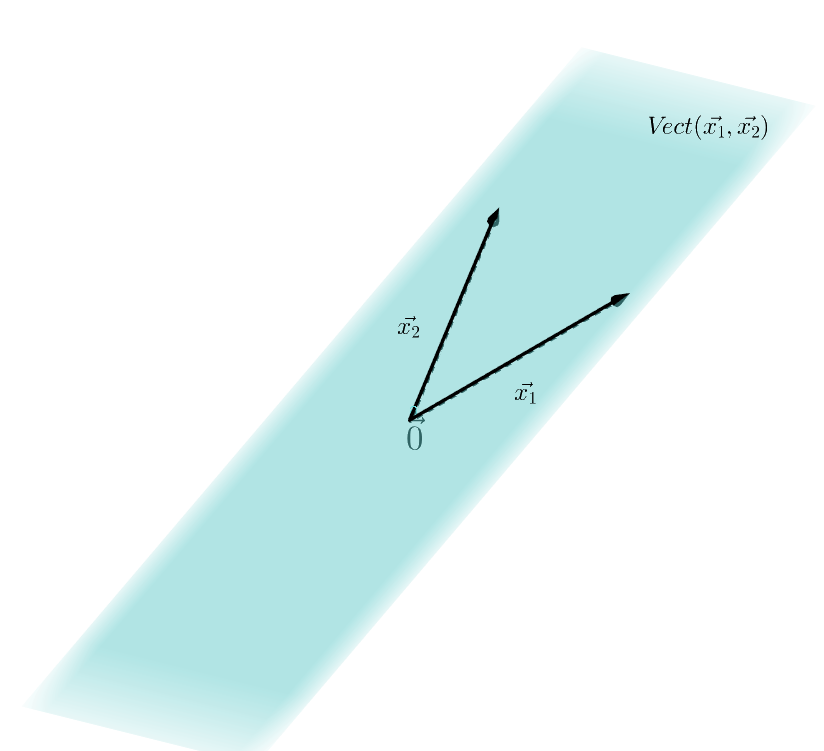
\includegraphics[width=6cm]{espace_vectoriel_plan.png}
\end{center}
\end{Exemple}
\subsubsection{Intersection $F_1\cap F_2$}

\begin{Proposition}
Soit $E$ un $\K $-espace vectoriel, $F_1, \dots, F_p$ des sous espaces vectoriels de $E$.\\
Alors l'intersection $\cap_{i=1}^p F_i$ est également un sous espace vectoriel.
\end{Proposition}
\begin{Demonstration}
\begin{itemize}
\item \textit{non vide :}\\
$\forall i \in \Intf{1}{p}: \Vect{0}\in F_i$ donc $\Vect{0}\in \cap_{i=1}^p F_i$
\item \textit{stable par $+$ :}\\
Soit $\Vect{x}_1,\Vect{x}_2 \in \cap_{i=1}^p F_i $ d'où pour tout $i\in \Intf{1}{p}: \Vect{x}_1,\Vect{x}_2\in F_i$.\\
Ainsi pour tout $i \in \Intf{1}{p}: \Vect{x}_1+\Vect{x}_2 \in F_i$ donc $\Vect{x}_1+\Vect{x}_2\in \cap_{i=1}^p F_i$.
\item
  \textit{stable par $.$ :} \\
Soit $\lambda\in \R$ et Soit $\Vect{x}\in \cap_{i=1}^p F_i $ d'où $\forall i \in \Intf{1}{p}: \Vect{x}\in F_i$.\\
Ainsi pour tout $i \in \Intf{1}{p}: \lambda\Vect{x}\in F_i$ donc $\lambda \Vect{x}\in \cap_{i=1}^p F_i$.
\end{itemize}
\end{Demonstration}
\begin{Exemple}$F=\overbrace{\{(x,y,z)\in \R^3: z=0\}}^{=F_1}\cap \overbrace{\{(x,y,z)\in \R^3: z=x\}}^{=F_2} $  l'intersection de deux plans vectoriels, $F_1$ et $F_2$ dans $\R ^3$
\begin{center}
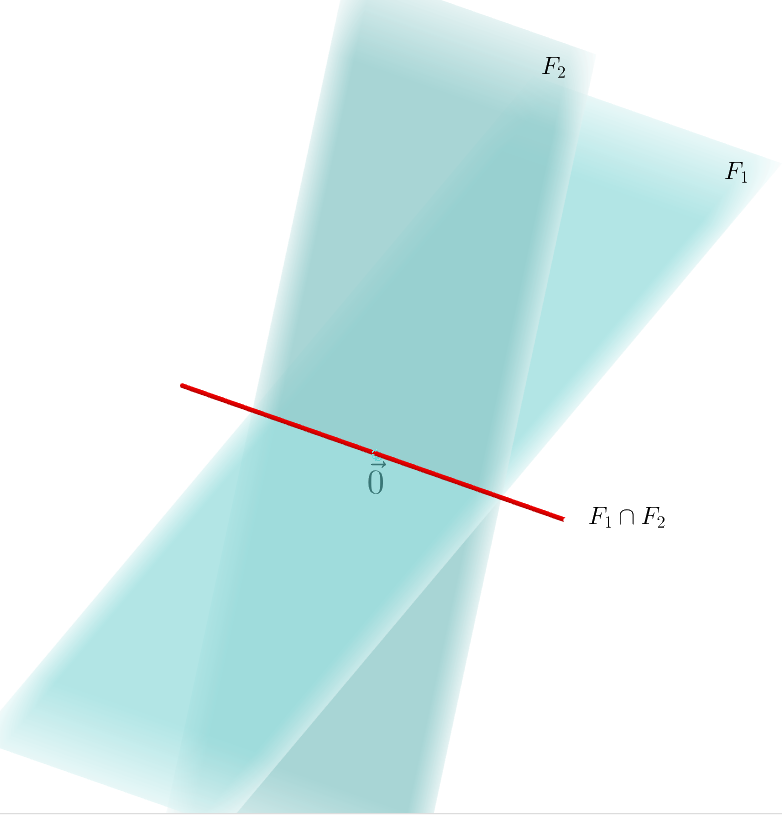
\includegraphics[width=6cm]{espace_vectoriel_inter.png}
\end{center}
\end{Exemple}

\subsubsection{Somme de sous-espaces vectoriels : $F_1+F2=\{\vec{x}+\vec{y}:\vec{x} \in F_1,\vec{y} \in F_2  \}$ }
\begin{Remarque}
L'union $\cup_{i=1}^p F_i$ n'est presque jamais un sous espace vectoriel.

\begin{center}
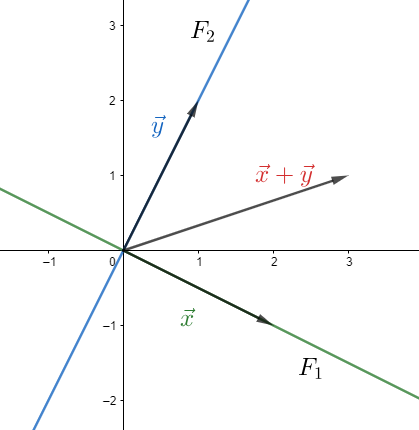
\includegraphics[width=4.5cm]{espace_vectoriel_union.png}
\end{center}
Sur cette figure, les vecteurs $\Vect{x},\Vect{y}\in F_1\cup F_2$ et on a $\Vect{x}+\Vect{y}\not\in  F_1 \cup F_2.$ La somme permet de construire le plus petit (au sens de l'inclusion) sous espace vectoriel  de $E$ contenant $F_1$ et $F_2$.
\end{Remarque}
\begin{DefinitionProposition}[Somme]
Soit $E$ un $\K $-espace vectoriel, $F_1$ et $F_2$ deux sous-espaces vectoriels de $E$.\\
On appelle \defi{somme} de $F_1$ et $F_2$ l'ensemble $ F_1+F_2$ des vecteurs de la forme $\Vect{x} +\Vect{y}$
où $\Vect{x}\in F_1$ et $\Vect{y}\in F_2$;
autrement dit,
\[  F_1+F_2 = \{\Vect{x} +\Vect{y} : \Vect{x}\in F_1,\Vect{y}\in F_2\}. \]
$F_1+F_2$ est un sous espace vectoriel  de $E$.\\
Plus précisément $F_1+F_2$ est le plus petit (au sens de l'inclusion) sous espace vectoriel  de $E$ contenant $F_1$ et $F_2$.
\end{DefinitionProposition}
\begin{Demonstration}
\begin{itemize}
\item \textit{non vide :}\\
$\Vect{0}\in F_1,F_2$ d'où $\Vect{0}=\underbrace{\Vect{0}}_{\in F_1}+\underbrace{\Vect{0}}_{\in F_2}\in F_1+F_2.$
\item \textit{stable par $+$ :}\\
Soit $\Vect{x_1}+\Vect{y_1},\Vect{x_2}+\Vect{y_2} \in  F_1+F_2.$\\
$\Vect{x_1}+\Vect{y_1}+\Vect{x_2}+\Vect{y_2} =\underbrace{\Vect{x_1}+\Vect{x_2}}_{\in F_1}+\underbrace{\Vect{y_1}+\Vect{y_2}}_{\in F_2}\in  F_1+F_2.$
\item
  \textit{stable par $.$ :} \\
Soit $\lambda\in \R$ et $\Vect{x}+\Vect{y}  \in  F_1+F_2.$\\
$\lambda (\Vect{x}+\Vect{y})=\underbrace{\lambda\Vect{x}}_{\in F_1}+\underbrace{\lambda\Vect{y}}_{\in F_2} \in  F_1+F_2.$
\end{itemize}
\end{Demonstration}
\begin{Exemple}
Soit $\R \Vect{x}_1$ et $\R \Vect{x}_2$ deux droite vectorielles distinctes. La somme de ces deux espace vectoriels forme le plan vectoriel $\R \Vect{x}_1+\R \Vect{x}_2$.
\begin{center}
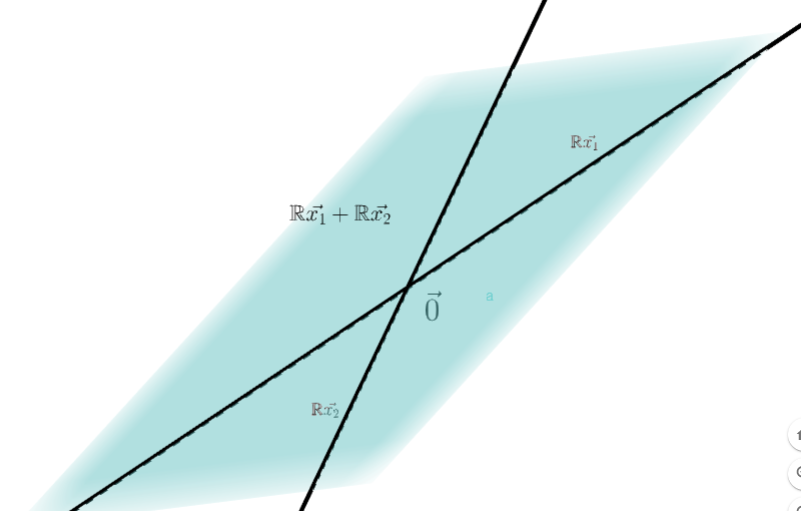
\includegraphics[width=8cm]{espace_vectoriel_somme.png}
\end{center}
\end{Exemple}

\begin{Definition}[Somme directe]
Avec les mêmes notations, on dit que la somme $F_1+F_2$ est \defi{directe} si tout vecteur de la somme se décompose \impo{de façon unique} sous la forme $\Vect{x} +\Vect{y}$ où $\Vect{x}\in F_1$ et $\Vect{y}\in F_2$.
On note alors la somme $F_1\oplus F_2$.
\end{Definition}
\begin{Proposition}[Critère 1]
Avec les mêmes notations, la somme $F_1+F_2$ est directe si et seulement si
$$ \forall \Vect{x} \in F_1, \forall \Vect{y} \in F_2:\quad 
  \Vect{x} +\Vect{y} = \Vect{0_E} \Rightarrow \Vect{x} =  \Vect{y} = \Vect{0_E}.$$
\end{Proposition}
\begin{Demonstration}$\quad$\\
\begin{itemize}
\item \textit{$(\Longrightarrow)$} :\\
Soit $\Vect{x} \in F_1$ et $\Vect{y} \in F_2$ tel que $\Vect{x} + \Vect{y}=\Vect{0}$. On a aussi $\underbrace{\Vect{0}}_{\in F_1}+\underbrace{\Vect{0}}_{\in F_2}=\Vect{0}.$ L'unicité de décomposition permet d'identifier  $\Vect{x}=\Vect{0}$ et $\Vect{y}=\Vect{0}$.
\item \textit{$(\Longleftarrow)$} :\\
Supposons qu'un $\Vect{z} \in F_1+F_2$  se décompose de 2 façons :$\Vect{z}= \underbrace{\Vect{x}}_{\in F_1} + \underbrace{\Vect{y}}_{\in F_2}$ et $\Vect{z}= \underbrace{\Vect{x'}}_{\in F_1} + \underbrace{\Vect{y}}_{\in F_2}$. \\
On soustrait ces deux égalités :
$$\Vect{0}= \underbrace{\Vect{x} -\Vect{x'} }_{\in F_1}+\underbrace{\Vect{y} -\Vect{y'} }_{\in F_2}.$$
D'après l'hypothèse, on a   $\Vect{x} -\Vect{x'}=\Vect{0}$ et $\Vect{y} -\Vect{y'}=\Vect{0}$, d'où l'unicité de la décomposition avec $\Vect{x} =\Vect{x'}$ et $\Vect{y}=\Vect{y'}.$ 
\end{itemize}
\end{Demonstration}
\begin{Proposition}[Critère 2]
Avec les mêmes notations, la somme $F_1+F_2$ est directe si et seulement si $F_1\cap F_2 = \{\Vect{0_E}\}$.
\end{Proposition}
\begin{Demonstration}$\quad $\\
\label{Proof:critere2}
\begin{itemize}
\item \textit{$(\Longrightarrow)$ :}
\begin{itemize}[label=*]
\item \textit{$\{\Vect{0_E}\}   \subset  F_1\cap F_2$} :
$\Vect{0_E}\in F_1,F_2$ donc $\Vect{0_E}\in F_1\cap F_2 .$ 
\item \textit{$F_1\cap F_2  \subset \{\Vect{0_E}\} $} :
Soit $\Vect{x}\in F_1\cap F_2$. 
On a $\Vect{0}= \underbrace{\Vect{x}}_{\in F_1} + \underbrace{-\Vect{x}}_{\in F_2}= \underbrace{\Vect{0}}_{\in F_1} + \underbrace{\Vect{0}}_{\in F_2}$. Par unicité de la décomposition, on identifie $\Vect{x}=\Vect{0}.$
\end{itemize}
Du fait de la double inclusion, on a $F_1\cap F_2 = \{\Vect{0_E}\}.$\\
\item \textit{$(\Longleftarrow)$ :}\\
Supposons qu'un $\Vect{z} \in F_1+F_2$  se décompose de 2 façons :$\Vect{z}= \underbrace{\Vect{x}}_{\in F_1} + \underbrace{\Vect{y}}_{\in F_2}$ et $\Vect{z}= \underbrace{\Vect{x'}}_{\in F_1} + \underbrace{\Vect{y}}_{\in F_2}$. \\
On soustrait ces deux égalités :
$$\underbrace{\Vect{x} -\Vect{x'} }_{\in F_1}=\underbrace{\Vect{y} -\Vect{y'} }_{\in F_2}.$$
Comme $F_1\cap F_2 = \{\Vect{0_E}\}$, on a $\Vect{x} -\Vect{x'}=\Vect{0}$ et $\Vect{y} -\Vect{y'} =\Vect{0}$, d'où l'unicité de la décomposition avec $\Vect{x} =\Vect{x'}$ et $\Vect{x}=\Vect{y'}.$
\end{itemize}

\end{Demonstration}

\begin{Exemple} Géométriquement, l'intersection entre deux plans vectoriels distincts, $F_1$ et $F_2$, est une droite vectoriel, $F_1\cap F_2$, donc la somme n'est pas directe.
\begin{center}
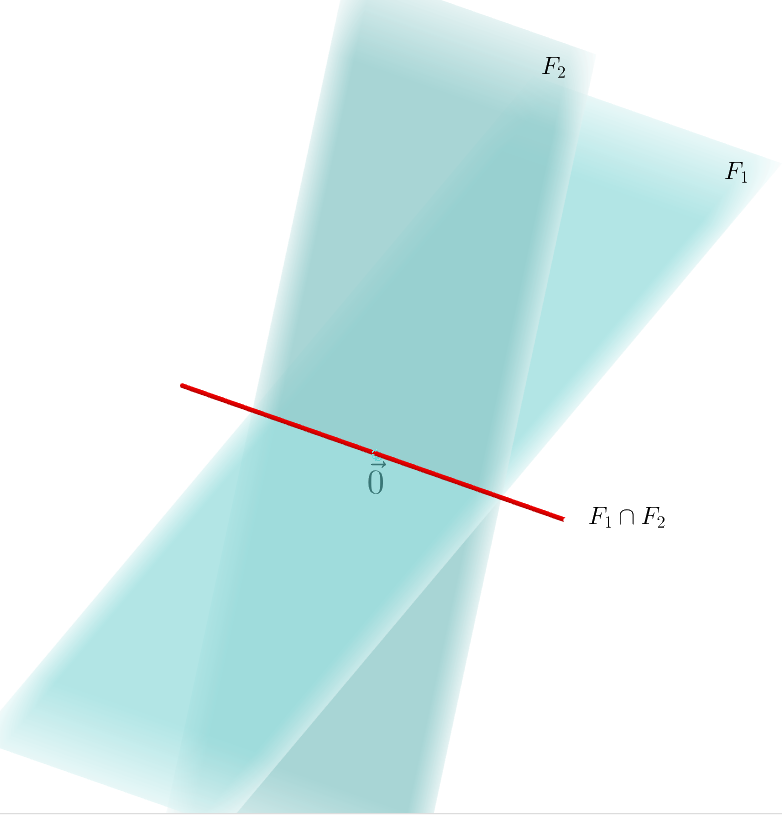
\includegraphics[width=6cm]{espace_vectoriel_inter.png}
\end{center}
Si $F_1=\{(x,y,z)\in\R^3: x+y+z=0\}$ et $F_1=\{(x,y,z)\in\R^3: x-y+z=0\}$. On a :
$$\begin{aligned}
 \Vect{x}=(x,y,z)\in F_1 \cap F_2 & \Leftrightarrow \begin{cases}x+y+z=0 \\ x-y+z=0 \end{cases}\\
 & \Leftrightarrow \begin{cases}x+y+z=0 \\ -2y=0 \quad L_2\leftarrow L_2 - L_1\end{cases}\\
 & \Leftrightarrow \begin{cases}x+z=0 \\ y=0 \end{cases}\\
 & \Leftrightarrow  z=\lambda, x=-\lambda , y=0,\quad  \forall t\in \R \\
 & \Leftrightarrow  (x,y,z) = \lambda(-1,0,1),\quad  \forall t\in \R \\
 & \Leftrightarrow  (x,y,z) \in \Vectt( -1,0,1)
 \end{aligned}$$
Finalement  $F_1 \cap F_2 = \R  ( -1,0,1)$. 
\end{Exemple}
\begin{Definition}[Supplémentaires]
Avec les mêmes notations, si la somme $F_1+F_2$ est directe et égale à $E$,
on dit que $F_1$ et $F_2$ sont \defi{supplémentaires}, et on note
\[ E = F_1\oplus F_2. \]
\end{Definition}
\begin{Exemple}
Montrons que $\R_n[X]=\R_{n-1}[X]\oplus \Vectt(X^n)$.\\
\begin{itemize}
\item \textit{$\R_n[X]=\R_{n-1}[X]+ \Vectt(X^n) $} :\\
Soit $P =a_0+a_1 X+\dots+a_{n-1} X^{n-1}+a_{n} X^{n}\in \R_n[X].$
On a $$P =\overbrace{a_0+a_1 X+\dots+a_{n-1} X^{n-1}}^{\in \R_{n-1}[X]}+\overbrace{a_{n} X^{n}}^{\in \Vectt(X^n)}.$$
\item \textit{$\R_{n-1}[X]\cap  \Vectt(X^n)=\{\Vect{0}_{\R_n[X]}\}$ :}\\
Soit $P \in \R_{n-1}[X]\cap \Vectt(X^n)$.\\
Comme $P \in \R_{n-1}[X]$, on a $deg(P)<n$. Comme  $P \in \Vectt(X^n)$, on a $P=\lambda X^n$. Si $\lambda\neq 0$, on a $deg(P=\lambda X^n)=n$, d'où une contradiction.  Donc $P=0$.  
\end{itemize}
\end{Exemple}
\begin{DefinitionProposition}[Somme]
Soit $E$ un $\K$-espace vectoriel et $F_1,\dots, F_p$ des sous-espaces vectoriels de $E$.\\
On appelle \defi{somme} de $F_1,\dots, F_p$ l'ensemble $ \sum_{k=1}^p F_k$ des vecteurs de la forme $\Vect{x_1} +\Vect{x_2}+ \dots + \Vect{x_p}$
où $\Vect{x_1}\in F_1$, $\Vect{x_2}\in F_2$, ..., $\Vect{x_p}\in F_p$;
autrement dit,
\[  \sum_{k=1}^p F_k = \{ \Vect{x_1} +\Vect{x_2}+ \dots + \Vect{x_p}: \Vect{x_1}\in F_1,\Vect{x_2}\in F_2,\dots, \Vect{x_p}\in F_p\}. \]
Il s'agit d'un sous espace vectoriel  de $E$;
plus précisément $S$ est le plus petit (au sens de l'inclusion) sous espace vectoriel  de $E$ contenant $F_1,\dots, F_p$.
\end{DefinitionProposition}


\begin{Definition}[Somme directe]
Avec les mêmes notations, on dit que la somme $\sum_{i=1}^p F_i$ est \defi{directe} si tout vecteur de la somme se décompose \defi{de façon unique} sous la forme $\Vect{x_1} +\Vect{x_2}+ \dots + \Vect{x_p}$ où $\Vect{x_1}\in F_1$, $\Vect{x_2}\in F_2$, ..., $\Vect{x_p}\in F_p$.
On note alors la somme $\oplus_{k=1}^p F_k$.
\end{Definition}
\begin{Proposition}[Critère 1]
Avec les mêmes notations, la somme $\sum_{i=1}^p F_i$ est directe si et seulement si
$$\Vect{x_1}\in F_1, \Vect{x_2}\in F_2, ..., \Vect{x_p}\in F_p,
 \Vect{x_1} +\Vect{x_2}+ \dots + \Vect{x_p} = \Vect{0_E} \implies \Vect{x_1} =\dots=\Vect{x_p}= \Vect{0_E}.$$
\end{Proposition}  
\begin{Remarque}
Le critère 2 ne se généralise pas (simplement) pour $p > 2$.\\
$E = \R ^2$, $\Vect{x_1} = (1,0)$, $\Vect{x_2} = (0,1)$ et $\Vect{x_3} = (1,1)$.
On a $\R \Vect{x_1} \cap \R \Vect{x_2} = \R \Vect{x_1} \cap \R \Vect{x_3} = \R \Vect{x_2} \cap \R \Vect{x_3} = \{(0,0)\}$. Cependant la somme $\R \Vect{x_1} + \R \Vect{x_2} + \R \Vect{x_3}$ n'est pas directe car $(1,1)=1(1,1)$ et $(1,1)=1(1,0)+1(0,1).$ 
\end{Remarque}



\subsection{Espace vectoriel produit : $(\vec{x_1},\vec{x_2})\in E_1\times E_2$}
\begin{Definition}[Produit cartésien]
Soit $(E_1, +_1, ._1)$ et $(E_2, +_2, ._2)$ deux $\K $-espaces vectoriels.\\
On pose \[ E = E_1\times E_2 = \{ (\Vect{x_1},\Vect{x_2}) : \Vect{x_1}\in E_1, \Vect{x_2}\in E_2 \}. \]
$E$ est le \defi{produit cartésien} des ensembles $E_1, E_2$.\\
On définit la loi de composition interne $+$ sur $E$ par : 
$$\forall (\Vect{x_1},\Vect{x_2})\in E, (\Vect{y_1},\Vect{y_2})\in E,\quad (\Vect{x_1},\Vect{x_2})+(\Vect{y_1},\Vect{y_2}) =  (\Vect{x_1}+_1\Vect{y_1},\Vect{x_2}+_2\Vect{y_2}). $$
De même, on définit la loi de composition externe $.$ sur $E$ par:
$$\forall \lambda \in \K,\forall (\Vect{x_1},\Vect{x_2}) \in E,
 \lambda . (\Vect{x_1},\Vect{x_2}) =(\lambda ._1\Vect{x_1},\lambda ._2\Vect{x_2}).$$
 \end{Definition}
 \begin{Exemple}
Pour $p\in \N^*$ et $E$ un $\K $-espace vectoriel, on définit $E^p$ par \[ E^p = \prod_{k=1}^p E. \]
Notez le cas particulier $E = \K $, où $E^p=\K^p$.  
 \end{Exemple}
\begin{Proposition}
$E$ ainsi défini est un $\K $-espace vectoriel.
\end{Proposition}
\begin{Definition} 
On définit de manière analogue le $\K $-espace vectoriel $E$,  produit cartésien des ensembles $E_1, \dots, E_n$.  $(E_1, +_1, ._1)$, $(E_2, +_2, ._2)$, ..., $(E_p, +_p, ._p)$ de $\K $-espaces vectoriels $ E = \prod_{k=1}^p E_k = \{ (\Vect{x_1},\dots, \Vect{x_p}): \Vect{x_1}\in E_1, \dots, \Vect{x_p}\in E_p \}$.
\end{Definition}




% -----------------------------------------------------------------------------
\section{Base: $\forall \vec{x}\in E, \exists !(\lambda_1,\dots \lambda_p),\quad \vec{x} = \lambda_1 \vec{e_1}+\dots +\lambda_p \vec{e_p}$}
\subsection{Définition}
\subsubsection{Famille génératrice : existence}
\begin{Definition}[Famille génératrice] Une famille finie  $\mathcal{F}=(\Vect{e}_1,\dots,\Vect{e_p})$ est \defi{génératrice} de $E$ si tout vecteur de $E$ est combinaison linéaire de $\mathcal{F}$, c'est à dire si $\Vectt(\mathcal{F}) = E$, c'est à dire si 
\[ \forall \Vect{x} \in E,\exists \lambda_1,\dots,\lambda_p \in \K,\quad \Vect{x} = \lambda_1 \Vect{e_1}+ \lambda_2 \Vect{e_2}+\dots +\lambda_p \Vect{e_p}. \]
\end{Definition}
\begin{Exemple} La famille  $\{(1,1), (0,1), (1,-1)\}$  est génératrice de $\R^2$. En effet, soit $\Vect{x}=(x,y)\in\R^2$, on a :
$$(x,y)=\frac{x+y}{2}(1,1)+ \frac{x-y}{2} (1,-1).$$
En revanche,  la combinaison linéaire n'est pas unique car $(x,y)= x(1,1)+(y-1)(0,1).$
\end{Exemple}
\subsubsection{Famille libre : unicité}
\begin{Definition}[Famille libre]
Une famille finie  $\mathcal{F}=(\Vect{e}_1,\dots,\Vect{e_p})$ est \defi{libre} si tout vecteur appartenant à l'espace vectoriel engendré par la famille s'exprime de manière unique comme combinaison linéaire de la famille, c'est à dire si 
\[ \forall \Vect{x} \in \Vectt((\Vect{e}_1,\dots,\Vect{e_p}),\exists ! \lambda_1,\dots,\lambda_n \in \K,\quad \Vect{x} = \lambda_1 \Vect{e_1}+ \lambda_2 \Vect{e_2}+\dots +\lambda_p \Vect{e_p}. \]
Autrement dit aucun des vecteurs de la famille n'est combinaison linéaire des autres.
\end{Definition}
\begin{Proposition}[Critère]
Une famille finie  $\mathcal{F}=(\Vect{e}_1,\dots,\Vect{e_p})$ est libre si et seulement si la seule combinaison linéaire de $\mathcal{F}$ nulle est triviale, c'est à dire
$$ \forall \lambda_1,\dots,\lambda_p   \in \K,\quad  \lambda _1 \Vect{e_1}+\dots+\lambda _n \Vect{e_n} = \Vect{0_E} \Rightarrow \lambda _1=\lambda _2=\dots=\lambda_p= 0_\K  .$$
\end{Proposition}
\begin{Demonstration}
La démonstration est similaire au critère 2 de la somme directe (voir démonstration~\ref{Proof:critere2}).
\end{Demonstration}
\begin{Exemple}
Dans l'exemple précédent, on a démontré qu'un vecteur pouvait s'exprimer à l'aide de deux combinaisons linéaires distinctes. Avec ce dernier critère, la démonstration serait :\\
Soit $\lambda,\beta,\alpha \in \R$ tel que $$\lambda (1,1) + \beta  (0,1) + \alpha (1,-1)    =(0,0).$$
On a : 
$$ \begin{cases}\lambda +\alpha &=0\\\lambda+\beta-\alpha&=0\end{cases}\Rightarrow \begin{cases}\lambda &=1\\\ \alpha&=-1\\ \beta&=-2 \end{cases}.$$
On vérifie que $(1,1)-2(0,1)- (1,-1) =(0,0)$.
\end{Exemple}
\subsubsection{Base : existence et unicité}
\begin{Definition}
On dit que la famille $\mathcal{F}=(\Vect{e}_1,\dots,\Vect{e_p})$ est une \defi{base} de $E$ si elle est libre et génératrice.\\
De façon équivalente, la famille $(\Vect{e}_1,\dots,\Vect{e_p})$ est une base de $E$ si
\[ \forall \Vect{x}\in E, \exists !  \lambda_1,\dots,\lambda_p   \in \K ,\quad  \Vect{x} = \lambda_1 \Vect{e_1}+ \lambda_2 \Vect{e_2}+\dots +\lambda_p \Vect{e_p}. \]
\end{Definition}
\begin{Exemple}
L'espace vectoriel des polynôme de degré inférieur ou égal à $n$, $\K _n[X]$,  admet une base $(1,X,X^2,\dots,X^n)$, appelée base canonique.
\end{Exemple}
\begin{Exemple}
L'espace vectoriel des matrices carrés de taille $2$, $\Mn{2}{\R}$,  admet une base $(\begin{pmatrix}1,0\\0,0\end{pmatrix},\begin{pmatrix}0,1\\0,0\end{pmatrix},\begin{pmatrix}0,0\\1,0\end{pmatrix},\begin{pmatrix}0,0\\0,1\end{pmatrix} )$, appelée base canonique.
\end{Exemple} 
 
\begin{Remarque} On n'a pas unicité de la base. Par exemple pour $\K _n[X]$, avec les $x_i$ $n+1$ scalaires distincts, les polynômes de Lagrange 
$$ l_{i}(X)=\prod _{j=0,j\neq i}^{n}{\frac {X-x_{j}}{x_{i}-x_{j}}} $$
$$l_{i}(X)={\frac {X-x_{0}}{x_{i}-x_{0}}}\cdots {\frac {X-x_{i-1}}{x_{i}-x_{i-1}}}~{\frac {X-x_{i+1}}{x_{i}-x_{i+1}}}\cdots {\frac {X-x_{n}}{x_{i}-x_{n}}}$$   forment une base de $\K _n[X]$.
\end{Remarque}

\subsection{Existence d'une base}
\begin{Definition}[Dimension finie]
Soit $E$ un $\K $-espace vectoriel.\\
On dit que $E$ est \defi{de dimension finie} s'il existe une famille finie génératrice de $E$,
et \defi{de dimension infinie} sinon.
\end{Definition}
\begin{Exemple}
L'espace vectoriel des polynôme est de dimension infinie.\\
En revanche, l'espace vectoriel des polynôme de degré inférieur ou égal à $n$ est finie.
\end{Exemple}
\begin{Exemple}
L'espace vectoriel des fonctions continues réels est  de dimension infinie.
\end{Exemple}

\begin{Theoreme}[Théorème de la base incomplète]
Soit $E$ un espace vectoriel de dimension finie et $\mathcal{L}$ une famille libre de $E$.\\  
Alors il existe une base $\mathcal{B}$ de $E$ telle que $\mathcal{L}\subset \mathcal{B}$.
\end{Theoreme}
\begin{Demonstration}
La démonstration  repose sur l'algorithme suivant :\\
Soit la partie libre initiale $\mathcal{L}$.\\
Comme $E$ est un espace vectoriel de dimension finie, il existe une famille finie, $\mathcal{G}$, génératrice de $E$.\\
Tant que $\mathcal{L}$ n'est pas génératrice de $E$ :
\begin{enumerate}
\item Puisque $\mathcal{G}$ engendre $E$ et que $\mathcal{L}$ n'est pas génératrice de $E$, il existe un vecteur $\Vect{g}$ de $\mathcal{G}$ qui n'est pas une combinaison linéaire d'éléments de $\mathcal{L}$.
\item On remplace $\mathcal{L}$ par $\mathcal{L}\cup \{\Vect{g} \}$, qui est encore libre car le nouveau vecteur n'est pas une combinaison linéaire des précédents.
\end{enumerate}
La boucle se termine en un nombre fini d'étapes puisqu'on ajoute à chaque étape un élément de $\mathcal{G}$ différent des précédents et que $\mathcal{G}$ est fini. $\mathcal{L}$ est alors une partie génératrice, donc une base de $E$.
\end{Demonstration}
\begin{Theoreme}[Théorème de la base extraite]
Soit $E$ un espace vectoriel de dimension finie et $\mathcal{G}$ une famille génératrice de $E$. \\ 
Alors il existe une base $\mathcal{B}$ de $E$ telle que $\mathcal{B}\subset \mathcal{G}.$
\end{Theoreme}
\begin{Demonstration}
La démonstration est identique à la précédente exceptée que $\mathcal{L}=\emptyset$.
\end{Demonstration}

\subsection{Unicité du cardinal de la base}
\begin{Proposition}
Si $E$ est un espace vectoriel de dimension finie admettant une famille génératrice de $n$ vecteurs, alors toute famille de $n+1$ vecteurs est liée.
\end{Proposition}
\begin{Demonstration}
Démontrons cette proposition par récurrence.
\begin{itemize}
\item \textit{Initialisation} :\\
Soit $(\Vect{g}_1)$ une famille génératrice de $E$.\\
Soit $(\Vect{v}_1,\Vect{v}_2)$ une famille de $E$. Il existe $\lambda_1$ et $\lambda_2$ dans $\R$ tel que $\Vect{v}_1=\lambda_1 \Vect{g}_1$ et $\Vect{v}_2=\lambda_2 \Vect{g}_1$.\\
Si  $\lambda_1=\lambda_2=0$ alors la famille $(\Vect{v}_1=\Vect{0},\Vect{v}_2=\Vect{0})$ est liée.\\
Si $\lambda_1\neq 0$, alors $\Vect{v}_1=\frac{\lambda_2}{\lambda_1}\Vect{v}_2$. Les vecteurs sont colinéaires donc liées.\\
Idem si $\lambda_2\neq 0$.\\
\item \textit{Hérédité} :\\
Soit $(\Vect{g_1},\dots,\Vect{g_n})$ une famille génératrice de $E$.\\
Soit $(\Vect{v}_1, \Vect{v}_2,\dots \Vect{v}_{n+1})$ une famille de $n+1$ vecteurs de $E$.\\
Pour tout $i\in \Intf{1}{n+1}$, il existe $\lambda_{i,1},\lambda_{i,2},\dots,\lambda_{i,n}\in\K$ tel que $$\Vect{v}_i=  \lambda_{i,1}\Vect{g}_1 + \lambda_{i,2}\Vect{g_2}+\dots+\lambda_{i,n}.\Vect{g_n}$$
Quitte à réorganiser les deux familles, on peut supposer que $\lambda_{n+1,n}\neq 0$. \\
Pour tout  $i\in \Intf{1}{n}$, on a 
$$\Vect{v}_i-\frac{\lambda_{i,n}}{\lambda_{n+1,n}}\Vect{v}_{n+1}\in \Vectt(\Vect{g_1},\dots,\Vect{g}_{n-1}).$$
On applique l'hypothèse de récurrence à l'espace vectoriel générée par la famille $(\Vect{g_1},\dots,\Vect{g}_{n-1})$. Donc la famille $\left(\Vect{v}_1-\frac{\lambda_{1,n}}{\lambda_{n+1,n}}\Vect{v}_{n+1},\dots, \Vect{v}_n-\frac{\lambda_{n,n}}{\lambda_{n+1,n}}\Vect{v}_{n+1}\right)$ est liée. Il existe  $\beta_{1},\beta_{2},\dots,\beta{n}\in\K$ non tous nuls tel que :
$$\beta_1 (\Vect{v}_1-\frac{\lambda_{1,n}}{\lambda_{n+1,n}}\Vect{v}_{n+1})+\dots+\beta_n (\Vect{v}_n-\frac{\lambda_{n,n}}{\lambda_{n+1,n}}\Vect{v}_{n+1})=\Vect{0}.$$
d'où 
$$\beta_1\Vect{v}_1+\dots +\beta_n\Vect{v}_n - (\beta_1\frac{\lambda_{1,n}}{\lambda_{n+1,n}}+\dots +\beta_n\frac{\lambda_{n,n}}{\lambda_{n+1,n}})\Vect{v}_{n+1}=\Vect{0}.$$
La famille est donc liée. 
\end{itemize}
\end{Demonstration}
\begin{Proposition}
Si $E$ est un espace vectoriel de dimension finie admettant une famille génératrice de $n$ vecteurs, alors toute famille ayant strictement plus de $n$ vecteurs est liée.
\end{Proposition}
\begin{Demonstration}
Si la famille a strictement plus de $n$ vecteurs, on peut en enlever pour constituer une famille de $n+1$ vecteurs qui est donc liée d'après la proposition précédente. A fortiori, la famille initiale est liée. 
\end{Demonstration}

\begin{Proposition}[Unicité du cardinal d'une base]
Soit $E$ un espace vectoriel de dimension finie et $(\Vect{e}_1,\dots,\Vect{e_p})$ et $(\Vect{f}_1,\dots,\Vect{f_q})$ deux bases de $E$.\\
Alors $p=q$.
\end{Proposition}
\begin{Demonstration}
$(\Vect{e}_1,\dots,\Vect{e_p})$ est une famille génératrice de $E$. Comme $(\Vect{f}_1,\dots,\Vect{f_q})$ est libre d'après la proposition précédente,  $q\leq p$.
Par symétrie, on a aussi $p\leq q$. Finalement $p=q$.
\end{Demonstration}
Cette proposition nous permet cette définition.
\begin{DefinitionProposition}[Dimension]
La \defi{dimension} d'un espace vectoriel de dimension finie est égale au cardinal d'une base quelconque de $E$.
\end{DefinitionProposition}

\begin{Proposition}[Critère]
Soit $E$ un espace vectoriel de dimension $n$.\\
Si $(\Vect{e}_1,\dots,\Vect{e_n})$ est une famille libre, alors $(\Vect{e}_1,\dots,\Vect{e_n})$ est une base de $E$.\\
Si $(\Vect{e}_1,\dots,\Vect{e_n})$ est une famille génératrice, alors $(\Vect{e}_1,\dots,\Vect{e_n})$ est une base de $E$.
\end{Proposition}
\begin{Exemple} Pour tout polynôme $P$ appartenant à $\K _{n}[X]$, la combinaison linéaire des polynômes de Lagrange  $\sum _{j=0}^{n}P(x_{j})l_{j}(X)$ avec $x_{0},\ldots ,x_{n}$ $n + 1$ scalaires distincts  est égale au polynôme $P$ aux points $x_{0},\ldots ,x_{n}$, donc égal à $P$. Les polynômes de Lagrange forment une famille génératrice de $n+1$ vecteurs. Comme $\dim(\K _{n}[X])=n+1$, ils forment une base de $\K _{n}[X]$. 
\end{Exemple}

\begin{Proposition}
Soit $E$ un espace vectoriel de dimension finie et $F$ un sous espace vectoriel de $E$.\\
Alors $F$ est également de dimension finie et $\dim F \leq \dim E$, avec égalité si et seulement si $F = E$.
\end{Proposition}

\subsection{Base adaptée}

\begin{Definition}[Base adaptée]
Soit $E$ un $\K $-espace vectoriel de dimension  $n$ et $F$ un sous espace vectoriel de $E$.\\
La base $(\Vect{e}_1,\dots,\Vect{e_n})$ est dite \defi{adaptée} à $F$
si et seulement s'il existe $p\in \Intf{1}{n}$ tel que $(\Vect{e}_1,\dots,\Vect{e_p})$ soit une base de $F$.
\end{Definition}
\begin{Exemple} La base $((1,-1,0),(0,1,-1),(0,0,1))$ est adaptée à $F=\{(x,y,z)\in\R ^3: x+y+z=0\}$ dans l'espace vectoriel $\R ^3$ car $((1,-1,0),(0,1,-1))$ est une base de $F$. 
\end{Exemple}
\begin{Proposition}[Existence d'une base adaptée]
La base ainsi définie existe.
\end{Proposition}
\begin{Demonstration}
Comme $F$ est un espace vectoriel de dimension finie, il existe une base $(\Vect{e}_1,\dots,\Vect{e_p})$ de $F$. Cette famille est libre dans $E$. On la complète en une base de $E$ d'après le théorème de la base incomplète.  
\end{Demonstration}
\begin{Definition}
Soit $E$ un $\K $-espace vectoriel de dimension finie, $F_1,\dots, F_p$ des sous-espaces vectoriels supplémentaires de $E$ et $B$ une base de $E$.\\
La base $\mathcal{B}$ est dite \defi{adaptée} à la décomposition $E =\oplus_{k=1}^p F_k$ si et seulement si $\mathcal{B}$ peut s'écrire comme la concaténation de $\mathcal{B}_1,\dots,\mathcal{B}_p$ où $\mathcal{B}_k$ est une base de $F_k$ pour tout $k\in \Intf{1}{p}$.
\end{Definition}
\begin{Proposition}
 La base ainsi définie existe.
\end{Proposition}
\begin{Proposition}
\label{prop:base}
Soit $E$ un $\K $-espace vectoriel de dimension finie et $\mathcal{B}$ une base de $E$.\\
On suppose que $\mathcal{B}$ s'écrit comme la concaténation de $\mathcal{B}_1,\dots \mathcal{B}_p$.\\
Pour $k\in \Intf{1}{p}$, notons $F_k$ le sous espace vectoriel engendré par $\mathcal{B}_k$.\\
Alors les sous-espaces vectoriels $F_1,\dots, F_p$ sont supplémentaires.
\end{Proposition}

\section{Théorèmes en dimension finie}
\begin{Proposition}[Existence d'un supplémentaire]
Dans un espace vectoriel de dimension finie, tout sous espace vectoriel admet un supplémentaire.\\
Autrement dit, soit $E$ est un espace vectoriel de dimension finie et $F$ un sous espace vectoriel de $E$.\\
Alors il existe un sous espace vectoriel $G$ de $E$ tel que $E = F \oplus G$.
\end{Proposition}
\begin{Demonstration}
Soit $\mathcal{B}_1$ une base de $F$ que l'on complète avec $\mathcal{B}_2$ pour former une base de $E$.\\
D'après la proposition \ref{prop:base}, si on pose $G$ l'espace vectoriel engendrée par  $\mathcal{B}_2$, alors $E = F \oplus G$.  
\end{Demonstration}
\begin{Proposition}
Soit $E_1,\dots E_p$ des $\K $-espaces vectoriels.\\
L'espace vectoriel produit $\prod_{k=1}^p E_k$ est de dimension finie si et seulement si $\forall k\in \Intf{1}{p}$, $E_k$ est de dimension finie.\\
De plus, dans ce cas, \[ \dim( \prod_{k=1}^p E_k ) = \sum_{k=1}^p \dim(E_k). \]
\end{Proposition}
\begin{Demonstration}
On suppose $p=2$.\\
Soit $(\Vect{e_1},\dots,\Vect{e_n})$ une base de $E_1$ et $(\Vect{f_1},\dots,\Vect{f_q})$ une base de $E_2$.\\
Alors $( (\Vect{e_1},\Vect{0}_F),\dots,(\Vect{e_n},\Vect{0}_F),(\Vect{0}_E,\Vect{f_1}),\dots,(\Vect{0}_E,\Vect{f_q}))$ est une base de $E_1\times E_2.$
\begin{itemize}
\item \textit{Génératrice} :\\
Soit $(\Vect{x},\Vect{y})\in E_1\times E_2$. \\
Comme $\Vect{x}\in E_1$ et $(\Vect{e_1},\dots,\Vect{e_n})$ est une famille génératrice de $E_1$, il existe $\lambda_1,\dots,\lambda_n\in \K$ tel que $\Vect{x}=\lambda_1\Vect{e_1}+\dots+ \lambda_n\Vect{e_n}$.\\
Comme $\Vect{y}\in E_2$ et $(\Vect{f_1},\dots,\Vect{f_q})$ est une famille génératrice de $E_2$, il existe $\beta_1,\dots,\beta_q\in \K$ tel que $\Vect{y}=\beta_1\Vect{f_1}+\dots+ \beta_q\Vect{f_q}$.\\
D'où $(\Vect{x},\Vect{y})=\lambda_1(\Vect{e_1},\Vect{0}_F)+\dots+\lambda_n(\Vect{e_n},\Vect{0}_F)+ \beta_1(\Vect{0}_E,\Vect{f_1})+\dots+\beta_q(\Vect{0}_E,\Vect{f_q}).$
\item \textit{Libre} :\\
Soit  $\lambda_1,\dots,\lambda_n,\beta_1,\dots,\beta_q\in \K$ tel que $$\lambda_1(\Vect{e_1},\Vect{0}_F)+\dots+\lambda_n(\Vect{e_n},\Vect{0}_F)+ \beta_1(\Vect{0}_E,\Vect{f_1})+\dots+\beta_q(\Vect{0}_E,\Vect{f_q})=(\Vect{0}_E,\Vect{0}_F).$$
D'où:
$$(\lambda_1\Vect{e_1}+\dots+ \lambda_n\Vect{e_n},\beta_1\Vect{f_1}+\dots+ \beta_q\Vect{f_q} )=(\Vect{0}_E,\Vect{0}_F).$$
Par identification, on obtient $\lambda_1\Vect{e_1}+\dots+ \lambda_n\Vect{e_n}=\Vect{0}_E$ et $\beta_1\Vect{f_1}+\dots+ \beta_q\Vect{f_q}=\Vect{0}_F$. Comme $(\Vect{e_1},\dots,\Vect{e_n})$ et $(\Vect{f_1},\dots,\Vect{f_q})$ sont des familles libres de $E_1$ et  de $E_2$ respectivement, $\lambda_1=\dots=\lambda_n=\beta_1=\dots=\beta_q=0$. 
\end{itemize}
\end{Demonstration}

\begin{Corollaire}
Pour $p\in \N^*$ et $E$ un $\K $-espace vectoriel.\\
L'espace vectoriel $E^p$ est de dimension finie si et seulement si $E$ l'est;
dans ce cas, on a $\dim(E^p) = p.\dim(E)$.
\end{Corollaire}
\begin{Proposition}[Formule de Grassmann]
Soit E un $\K $-espace vectoriel dimension finie et $F_1$, $F_2$ deux sous espace vectoriel de $E$. On a :
$$\dim (F_1 + F_2) = \dim F_1 + \dim F_2 - \dim(F_1 \cap F_1).$$
\end{Proposition}
\begin{Demonstration}
Une idée est de remarquer l'analogie avec la formule ensembliste  :
$$\text{card}(A)+\text{card}(B)=\text{card}(A\cup B)+\text{card}(A\cap B).$$
Soit $(\Vect{e_1},\dots,\Vect{e_p})$ une base de $F_1\cap F_2$. On la complète en une base 
$(\Vect{e_1},\dots,\Vect{e_p},\Vect{f_{p+1}},\dots,\Vect{f_{p+k}})$ de $F_1$ et en une base $(\Vect{e_1},\dots,\Vect{e_p},\Vect{g_{p+1}},\dots,\Vect{g_{p+m}})$ de $F_2$. $(\Vect{e_1},\dots,\Vect{e_p},\Vect{f_{p+1}},\dots,\Vect{f_{p+k}},\Vect{g_{p+1}},\dots,\Vect{g_{p+m}})$ est une base   $F_1+F_2$.\\
Comme le cardinal d'une base est égale à la dimension de l'espace vectoriel, on obtient bien l'égalité souhaitée.
\end{Demonstration}
\begin{Proposition}
Soit $E$ un $\K $-espace vectoriel et $F_1,\dots F_p$ des sous-espaces vectoriels de dimension finie de $E$.
Alors la somme $\sum_{k=1}^p F_k$ est également de dimension finie, et
\[ \dim\left(\sum_{k=1}^p F_k \right)  \leq \sum_{k=1}^p \dim(F_k). \]
De plus, il y a égalité si et seulement si la somme $\sum_{k=1}^p F_k$ est directe.
\end{Proposition}
\begin{Proposition}
Soit $E$ un $\K $-espace vectoriels de dimensions finies et $F_1, \dots, F_p$ des sous espaces vectoriels de $E$.\\
On suppose que \[ \sum_{k=1}^p \dim F_k = \dim E. \]
Les conditions suivantes sont alors équivalentes:
\begin{enumerate}
\item
 les sous espaces vectoriels $F_1, \dots, F_p$ sont supplémentaires,
\item
  les sous espaces vectoriels $F_1, \dots, F_p$ sont en somme directe,
\item  $\sum_{k=1}^p F_k = E$.
\end{enumerate}
\end{Proposition}
%TODO ECRIRE CETTE PARTIE
\section{Retour aux matrices}
\begin{Proposition}[Structure de $\K $-espace vectoriel]
$\MnpK$ possède une structure de $\K $-espace vectoriel. 
\end{Proposition}
\begin{Demonstration}
Tous les axiomes se vérifient aisément.  
\end{Demonstration}
\begin{DefinitionProposition}[Base canonique]La \defi{base canonique} est $(E_{ij})_{1\leqslant i\leqslant n, 1\leqslant j\leqslant p}$ où la matrice  $E_{i,j}$ est celle dont tous les coefficients sont nuls sauf celui d'indice $(i,j)$ , qui vaut 1.\\
 Les coordonnées dans la base canonique d'une matrice $A$ sont ses coefficients :
 $$ \begin{pmatrix}
a_{11} & \cdots & a_{1p}\\
 \vdots &  & \vdots\\
a_{n1} & \cdots & a_{np}
\end{pmatrix} =a_{11}\begin{pmatrix}
1 & \cdots & 0\\
 \vdots &  & \vdots\\
0 & \cdots & 0
\end{pmatrix}+\dots+a_{1p}\begin{pmatrix}
0 & \cdots & 1\\
 \vdots &  & \vdots\\
0 & \cdots & 0
\end{pmatrix}+ \dots+a_{n1}\begin{pmatrix}
0 & \cdots & 0\\
 \vdots &  & \vdots\\
1 & \cdots & 0
\end{pmatrix}+\dots+a_{np} \begin{pmatrix}
0 & \cdots & 0\\
 \vdots &  & \vdots\\
0 & \cdots & 1
\end{pmatrix},$$
 $$ \begin{pmatrix}
a_{11} & \cdots & a_{1p}\\
 \vdots &  & \vdots\\
a_{n1} & \cdots & a_{np}
\end{pmatrix} =  \sum _{1\leqslant i\leqslant n\atop 1\leqslant j\leqslant p}  a_{ij} E_{ij}.$$
On a $\dim( \MnpK)=np$.
\end{DefinitionProposition}
\begin{Demonstration}
Du fait de l'égalité, $ A = \sum _{1\leqslant i\leqslant n\atop 1\leqslant j\leqslant p}  a_{i,j} E_{i,j}$,  $(E_{i,j})_{1\leqslant i\leqslant n, 1\leqslant j\leqslant p}$ est une famille génératrice de $\MnpK$.\\
Soit  $(\lambda_{ij})_{1\leqslant i\leqslant n, 1\leqslant j\leqslant p}$ une famille de scalaires tel que
$$\sum _{1\leqslant i\leqslant n\atop 1\leqslant j\leqslant p}  \lambda_{ij} E_{i,j}=0_{\MnpK}.$$
D'où :
 $$\begin{pmatrix}
\lambda_{11} &  \cdots & \lambda_{1p}\\
\vdots & \ \ddots & \vdots\\
\lambda_{n1} &  \cdots & a_{np}\\
\end{pmatrix}= \begin{pmatrix}
0 &  \cdots &0\\
\vdots & \ \ddots & \vdots\\
0 &  \cdots & 0\\
\end{pmatrix}$$
Par identification, $\lambda_{ij}=0$ pour tout $i\in\Intf{1}{n}$ et  $j\in\Intf{1}{p}$, donc la famille est libre.\\
La famille est donc une base. Comme la cardinal de la base $\mathrm{Card}((E_{i,j})_{1\leqslant i\leqslant n, 1\leqslant j\leqslant p})$ est $np$, on a bien $\dim( \MnpK)=np$.
\end{Demonstration}
\begin{Exemple}$ \begin{pmatrix}
0 &1  \\
4 & 3 \\
\end{pmatrix} =
0\cdot
\begin{pmatrix}
1 &0  \\
0 & 0  \\
\end{pmatrix}
+
1\cdot
\begin{pmatrix}
0 &1  \\
0 & 0 \\
\end{pmatrix}
+
4\cdot
\begin{pmatrix}
0 &0  \\
1 & 0  \\
\end{pmatrix}
+
3\cdot
\begin{pmatrix}
0 &0  \\
0 & 1  \\
\end{pmatrix}
$
\end{Exemple}

\end{document}
